\documentclass[
	% -- opções da classe memoir --
	12pt,				% tamanho da fonte
	%openright,			% capítulos começam em pág ímpar (insere página vazia caso preciso)
	oneside,			% p/ impressão frente e verso:
	%					%oneside -> Normal. 
	%					%twoside -> insere página antes e depois de cada capítulo
	a4paper,			% tamanho do papel. 
	% -- opções da classe abntex2 --
	%chapter=TITLE,		% títulos de capítulos convertidos em letras maiúsculas
	%section=TITLE,		% títulos de seções convertidos em letras maiúsculas
	%subsection=TITLE,	% títulos de subseções convertidos em letras maiúsculas
	%subsubsection=TITLE,% títulos de subsubseções convertidos em letras maiúsculas
	% -- opções do pacote babel --
	english,			% idioma adicional para hifenização
	french,				% idioma adicional para hifenização
	spanish,			% idioma adicional para hifenização
	brazil				% o último idioma é o principal do documento
	]{abntex2}
% ---
% Pacotes básicos 
% ---
\usepackage{lmodern}			% Usa a fonte Latin Modern			
\usepackage[T1]{fontenc}		% Selecao de codigos de fonte.
\usepackage[utf8]{inputenc}		% Codificacao do documento (conversão automática dos acentos)
\usepackage{indentfirst}		% Indenta o primeiro parágrafo de cada seção.
\usepackage{color}				% Controle das cores
\usepackage{graphicx}			% Inclusão de gráficos
\usepackage{microtype} 			% para melhorias de justificação

% ---
% Atribuições Matemáticas 
% ---
\usepackage{amsmath, amsfonts, amssymb} % pacotes para caracteres extras
\DeclareMathOperator{\sen}{sen}
\DeclareMathOperator{\arcsen}{arcsen}
\DeclareMathOperator{\tg}{tg}
\DeclareMathOperator{\cossec}{cossec}
\newcommand{\limite}{\displaystyle\lim}
\newcommand{\integral}{\displaystyle\int}
		
% ---
% Pacotes de citações
% ---
\usepackage[brazilian,hyperpageref]{backref}	 % Paginas com as citações na bibl
\usepackage[alf]{abntex2cite}	% Citações padrão ABNT

% --- 
% CONFIGURAÇÕES DE PACOTES
% --- 

% ---
% Configurações do pacote backref
% Usado sem a opção hyperpageref de backref
\renewcommand{\backrefpagesname}{Citado na(s) página(s):~}
% Texto padrão antes do número das páginas
\renewcommand{\backref}{}
% Define os textos da citação
\renewcommand*{\backrefalt}[4]{
	\ifcase #1 %
		Nenhuma citação no texto.%
	\or
		Citado na página #2.%
	\else
		Citado #1 vezes nas páginas #2.%
	\fi}%
% ---

% ---
% Informações de dados para CAPA e FOLHA DE ROSTO
% ---
\titulo{TRABALHO 2: \\ \textbf{Circuitos RL, RC e RLC}}
\autor{Antonio Gabriel Sousa Borralho \\ Antonio José Portela de Jesus Santos \\ Arthur Monteiro Costa Silva \\ Bruno Leal da Silva \\ Lucas Costa Soares}
\local{São Luís, MA - Brasil}
\data{\today}
%\orientador{Prof. Professor}
\tipotrabalho{Relatório Experimental}
% O preambulo deve conter o tipo do trabalho, o objetivo, 
% o nome da instituição e a área de concentração 
\preambulo{Trabalho referente à resolução das questões da segunda lista de exercícios, para obtenção parcial da segunda nota da disciplina Circuitos Elétricos.\newline \newline Prof. Luciano Buonocore.}
% ---


% ---
% Configurações de aparência do PDF final

% alterando o aspecto da cor azul
\definecolor{blue}{RGB}{41,5,195}

% informações do PDF
\makeatletter

\hypersetup{
     	%pagebackref=true,
		pdftitle={\@title}, 
		pdfauthor={\@author},
    	%pdfsubject={\imprimirpreambulo},
	    pdfcreator={LaTeX with abnTeX2},
		pdfkeywords={abnt}{latex}{abntex}{abntex2}{trabalho acadêmico}, 
		colorlinks=true,       		% false: boxed links; true: colored links
    	linkcolor=blue,          	% color of internal links
    	citecolor=blue,        		% color of links to bibliography
    	filecolor=magenta,          % color of file links
		urlcolor=blue,
		bookmarksdepth=4
}

\makeatother
% --- 

% --- 
% Espaçamentos entre linhas e parágrafos 
% --- 

% O tamanho do parágrafo é dado por:
\setlength{\parindent}{1.3cm}

% Controle do espaçamento entre um parágrafo e outro:
\setlength{\parskip}{0.2cm}  % tente também \onelineskip

% ---
% compila o indice
% ---
\makeindex
% ---

% ----
% Início do documento
% ----
\begin{document}

% Seleciona o idioma do documento (conforme pacotes do babel)
%\selectlanguage{english}
\selectlanguage{brazil}

% Retira espaço extra obsoleto entre as frases.
\frenchspacing 

% ----------------------------------------------------------
% ELEMENTOS PRÉ-TEXTUAIS
% ----------------------------------------------------------
\pretextual
% ---
% --------------------- CAPA -------------------------------
% ---
\begin{center}			
	\begin{figure}[htb]
		\centering
		
\includegraphics[scale=0.15]{ufmalogo.jpg}
	\end{figure}
				
			\textbf{UNIVERSIDADE FEDERAL DO MARANHÃO \\
					CENTRO DE CIÊNCIAS EXATAS E TECNOLOGIAS \\
					DEPARTAMENTO DE ENGENHARIA ELÉTRICA \\
				    CIRCUITOS ELÉTRICOS\\\vspace{4cm}}
					
					\textbf{\large{TRABALHO 2:}\\
					\large{Circuitos RL, RC e RLC}}
					\vspace{3.5cm}
					\begin{flushright}
						\textnormal{Antonio Gabriel Sousa Borralho \\ Antonio José Portela de Jesus Santos \\ Arthur Monteiro Costa Silva \\ Bruno Leal da Silva \\ Lucas Costa Soares}
					\end{flushright}
					\vspace{3.5cm}
					\textbf{São Luís, MA - Brasil\\ \today}
\end{center}
% ---
% --------------------- FOLHA DE ROSTO -------------------------------
% ---
\renewcommand{\folhaderostocontent}{  % Cria sua própria folha de rosto 
    \begin{center}
        % ____Autores_________________________________________
        {\ABNTEXchapterfont\imprimirautor}
        \vspace*{\fill}\vspace*{\fill}
        % ____Título_________________________________________
        \begin{center}
            \ABNTEXchapterfont\bfseries\Large\imprimirtitulo
        \end{center}
        \vspace*{\fill}
        % ____Pré-Ambulo_________________________________________
        \abntex{}{%
            \hspace{.45\textwidth}
            \begin{minipage}{.5\textwidth}
                \SingleSpacing
                \imprimirpreambulo
            \end{minipage}%
            \vspace*{\fill}
        }%
        % ____Instituição_______________________________________
        %{\abntex{\imprimirinstituicao}{\imprimirinstituicao
        %\vspace*{\fill}}}
        % ____Orientador_________________________________________
        %{\large\imprimirorientadorRotulo~\imprimirorientador\par}
        % ____Co-Orientador___________________________________
        %\abntex{\imprimircoorientador}{%
        %    {\large\imprimircoorientadorRotulo~\imprimircoorientador}%
        %}%
        % ____Local/Data______________________________________
        {\large\imprimirlocal}
        \par
        {\large\imprimirdata}
        %\vspace*{1cm}
    \end{center}
}
\makeatother
% ---
% Folha de rosto
% (o * indica que haverá a ficha bibliográfica)
% ---
\imprimirfolhaderosto

% ---
% --------------------- SUMÁRIO -------------------------------
% ---
\pdfbookmark[0]{\contentsname}{toc}
\tableofcontents*
\cleardoublepage
% ---

% ----------------------------------------------------------
% ELEMENTOS TEXTUAIS
% ----------------------------------------------------------
\textual
% ----------------------------------------------------------
% Introdução (exemplo de capítulo sem numeração, mas presente no Sumário)
% ----------------------------------------------------------
\chapter{Conceitos Básicos}
% ----------------------------------------------------------

Circuitos com \textbf{resistores, capacitores e indutores} denominados $RL$, $RC$ ou $RLC$, que apesar de sua simplicidade, têm inúmeras aplicações em eletrônica, comunicação e sistemas de controle \cite{sadiku}. Assim como outros, esses componentes são mais fáceis de descrever em termos de variáveis de circuito do que de variáveis eletromagnéticas. No entanto, antes de nos concentrarmos na descrições desses elementos do ponto de vista de circuitos, é recomendável realizarmos uma breve revisão dos conceitos de campo a eles subjacentes. 

Um indutor é um componente elétrico que se opõe a qualquer mudança na corrente elétrica. É composto por uma bobina de fio enrolado em torno de um núcleo de suporte cujo material pode ser magnético ou não magnético. O comportamento dos indutores é baseado em fenômenos associado a campos magnéticos. Um  campo magnético que varia com o tempo induz uma tensão em qualquer condutor imerso ao campo. O parâmetro \textbf{indutância} relaciona a tensão induzida com a corrente. Um capacitor é um componente elétrico que consiste em dois condutores separados por um isolante ou material dielétrico. O capacitor é o único dispositivo, além da bateria, que pode armazenar carga elétrica. O comportamento dos capacitores é baseado em fenômenos associados a campos elétricos. Um campo elétrico que varia com o tempo produz uma corrente de deslocamento no espaço ocupado pelo campo. O parâmetro \textbf{capacitância} relaciona a corrente de deslocamento à tensão, onde a corrente de deslocamento é igual à corrente de condução nos terminais do capacitor.

A análise de circuitos $RL$ e $RC$ é dividida em três fases. Na primeira fase, examinamos as correntes e tensões que surgem quando a energia armazenada em um indutor ou capacitor é fornecida repentinamente a uma carga. Isso ocorre quando o indutor ou capacitor é desligado de forma abrupta de sua fonte cc. As correntes e tensões que surgem nessa configuração são denominadas \textbf{resposta natural} do circuito. Na segunda fase, examinaremos as correntes e tensões que surgem quando a energia é recebida por um indutor ou capacitor por causa da aplicação repentina de uma fonte de tensão ou corrente cc. Essa resposta é denominada \textbf{resposta a um degrau}. A terceira fase consiste em determinar um método geral que pode ser usado para determinar a resposta de circuitos $RL$ e $RC$ a qualquer variação abrupta em uma fonte de tensão ou corrente cc.

A discursão da resposta natural e da resposta a um degrau de circuitos que contém indutores e capacitores ($RLC$), está limitada a duas estruturas bem simples: O circuito $RLC$ em paralelo e o circuito $RLC$ em série.
\cite{nilssonriedel}
%=====================================================================================================================================================
%====== QUESTÕES ===============================================================================================================================================
\chapter{Questões}

% ----------------------------------------------------------
% QUESTÃO 2.1
% ----------------------------------------------------------

\section*{Questão 2.1}
\addcontentsline{toc}{section}{Questão 2.1}
Calcule a potência dissipada no resistor de $40\Omega$ e a tensão representada por $V_C$ em cada um dos Circuitos 2.1(a) e 2.1(b).
\begin{figure}[htb]
	\centering
	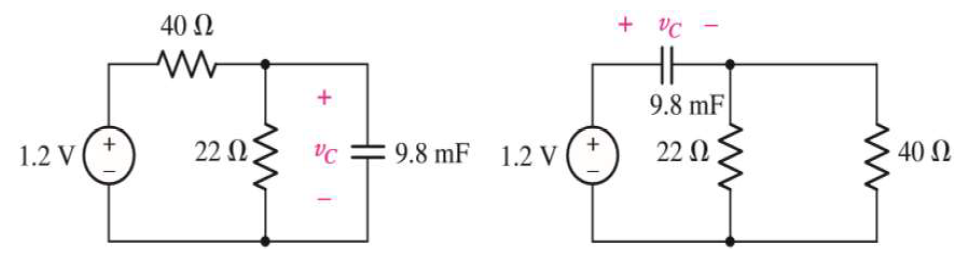
\includegraphics[scale=0.5]{2-1.PNG}
	\caption{Circuitos 2.1(a) e 2.1(b)}
\end{figure}

%--2.1 - Letra A -------------------------------------------------------------------------------------
$a)$ Observamos que o circuito está ligado por bastante tempo $(t\rightarrow \infty)$. Com isso, a corrente do capacitor é:
$$i_C = C\dfrac{d v_c}{dt}$$

Como o circuito está ligado por bastante tempo: $v_c$ é constante e $\dfrac{d v_c}{dt} = 0$, assim:
$$i_C = C\dfrac{d v_c}{dt} \Longrightarrow i_C = C \cdot 0 \Longrightarrow i_C=0A$$

Desta forma o capacitor é visto pelo circuito como \textcolor{red}{malha aberta}. Calculando $v_C$ e $v_{40\Omega}$ por \textbf{\textcolor{red}{divisor de tensão}}:
\begin{equation}
    \centering
    v_C = \dfrac{22\Omega}{40\Omega + 22\Omega} \cdot 1,2V \Longrightarrow \fbox{$v_C = 425,806\;mV$} 
\end{equation}

$$v_{40\Omega} = \dfrac{40\Omega}{40\Omega + 22\Omega} \cdot 1,2V = 774,194 \;mV$$

A potência no resistor de $40\Omega$ é:
$$P_{40\Omega} = \dfrac{v_{40\Omega}^2}{R_{40\Omega}} = \dfrac{774,194\;mV}{40}$$
\begin{equation}
    \centering
    \fbox{$P_{40\Omega} = 14,984\;mV$}
\end{equation}

%--2.1 - Letra B -------------------------------------------------------------------------------------
\newpage
$b)$ Observamos que o circuito está ligado por bastante tempo $(t\rightarrow \infty)$. Com isso, a corrente do capacitor é:
$$i_C = C\dfrac{d v_c}{dt}$$

Como o circuito está ligado por bastante tempo: $v_c$ é constante e $\dfrac{d v_c}{dt} = 0$, assim:
$$i_C = C\dfrac{d v_c}{dt} \Longrightarrow i_C = C \cdot 0 \Longrightarrow i_C=0\;A$$

Desta forma o capacitor é visto pelo circuito como malha aberta. Calculando $v_C$ \textbf{\textcolor{red}{pelo método das correntes de malha}}, temos:
$$-1,2 + v_C + 22\cdot I = 0$$

Como $I=0$,
\begin{equation}
    \centering
    \fbox{$v_C=1,2\;V$}
\end{equation}

Calculando a potência no resistor de $40\Omega$:
$$P_{40\Omega} = R\cdot i^2$$

Pelo circuito, temos que a corrente no resistor de $40\Omega$ é $0\;A$, portanto:
\begin{equation}
    \centering
    \fbox{$P_{40\Omega} = 40\cdot 0^2 = 0\;W$}
\end{equation}

\begin{flushright}
    $\Box$
\end{flushright}
\newpage
% ----------------------------------------------------------
% QUESTÃO 2.3
% ----------------------------------------------------------
\section*{Questão 2.3}
\addcontentsline{toc}{section}{Questão 2.3}
Calcule $v_L$ e $i_L$ para cada um dos circuitos mostrados abaixo, se $i_S = 1mA$ e $v_S = 2.1\;V$.

\begin{figure}[htb]
	\centering
	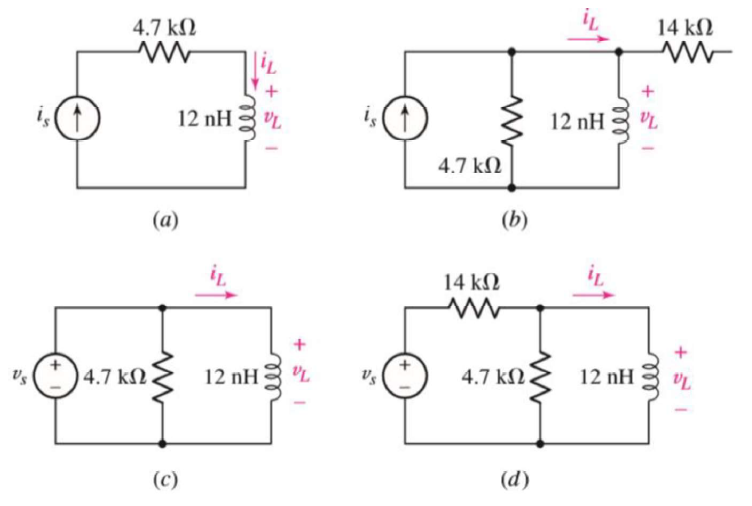
\includegraphics[scale=0.5]{2-3.PNG}
	\caption{Circuitos 2.3}
\end{figure}

%--2.3 - Letra A -------------------------------------------------------------------------------------
$a)$ $i_S = 1mA$ e $v_S=2,1V$

Como o circuito está ligado por bastante tempo, a corrente: $i_L$ é constante e $\dfrac{d i_L}{dt} = 0$, assim:
\begin{equation}
    \centering
    v_L = L\dfrac{d i_L}{dt} \Longrightarrow v_L = L \cdot 0 \Longrightarrow \fbox{$v_L = 0V$}
\end{equation}

Como não existe tensão nos terminais do indutor, ele pode ser substituído por um curto-circuito. Assim:
\begin{equation}
    \fbox{$i_L = i_S = 1\;mA$}
\end{equation}

%--2.3 - Letra B -------------------------------------------------------------------------------------
$b)$ Como o circuito está ligado por bastante tempo, a corrente: $i_L$ é constante e $\dfrac{d i_L}{dt} = 0$, assim:
\begin{equation}
    \centering
    v_L = L\dfrac{d i_L}{dt} \Longrightarrow v_L = L \cdot 0 \Longrightarrow \fbox{$v_L = 0V$}
\end{equation}

Como não existe tensão nos terminais do indutor, ele pode ser substituído por um curto-circuito. Assim:
\begin{equation}
    \fbox{$i_L = i_S = 1\;mA$}
\end{equation}

\newpage

%--2.3 - Letra C -------------------------------------------------------------------------------------
$c)$ Como o circuito está ligado por bastante tempo, a corrente: $i_L$ é constante e $\dfrac{d i_L}{dt} = 0$, assim:
\begin{equation}
    \centering
    v_L = L\dfrac{d i_L}{dt} \Longrightarrow v_L = L \cdot 0 \Longrightarrow \fbox{$v_L = 0\;V$}
\end{equation}

Como não existe tensão nos terminais do indutor, ele pode ser substituído por um curto-circuito. Desta forma encontramos uma resistência equivalente:
$$R_{eq} = \dfrac{4,7 \times 10^3 \cdot 0 \Omega}{4,7 \times 10^3 \Omega + 0 \Omega} = 0\Omega$$

\begin{equation}
    i_f = i_L =  \dfrac{2,1\;V}{0 \Omega} \Longrightarrow \fbox{$i_L \rightarrow \infty A$}
\end{equation}

%--2.3 - Letra D -------------------------------------------------------------------------------------
$d)$ Como o circuito está ligado por bastante tempo, a corrente: $i_L$ é constante e $\dfrac{d i_L}{dt} = 0$, assim:
\begin{equation}
    \centering
    v_L = L\dfrac{d i_L}{dt} \Longrightarrow v_L = L \cdot 0 \Longrightarrow \fbox{$v_L = 0\;V$}
\end{equation}

Como não existe tensão nos terminais do indutor, ele pode ser substituído por um curto-circuito. Desta forma o resistor de $4,7 k \Omega$ perde seu efeito, assim:
$$R_{eq} = 14 k \Omega$$


\begin{equation}
    i_f =  \dfrac{2,1 V}{14 \times 10^3 \Omega} = \fbox{$i_L = 150\;\mu A$}
\end{equation}

\begin{flushright}
    $\Box$
\end{flushright}
\newpage
% ----------------------------------------------------------
% QUESTÃO 2.5
% ----------------------------------------------------------
\section*{Questão 2.5}
\addcontentsline{toc}{section}{Questão 2.5}
Reduza o Circuito 2.5 para o menor número de componentes possível.

\begin{figure}[htb]
	\centering
	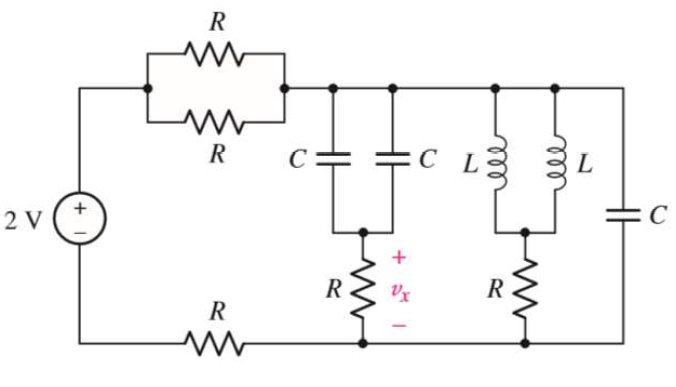
\includegraphics[scale=0.5]{2-5.PNG}
	\caption{Circuitos 2.5}
\end{figure}

Fazendo a associação dos resistores, temos:
\begin{equation}
    R_{eq} = \dfrac{R}{2} + R = \dfrac{R+2R}{2} = \dfrac{3R}{2} \Longrightarrow \fbox{$R_{eq} = 1,5R$}
\end{equation}

\begin{equation}
    C_{eq} = C+C \Longrightarrow \fbox{$C_{eq} = 2C$}
\end{equation}

\begin{equation}
    \fbox{$L_{eq} = \dfrac{L}{2}$}
\end{equation}

Obtemos assim o seguinte circuito equivalente:
\begin{figure}[htb]
	\centering
	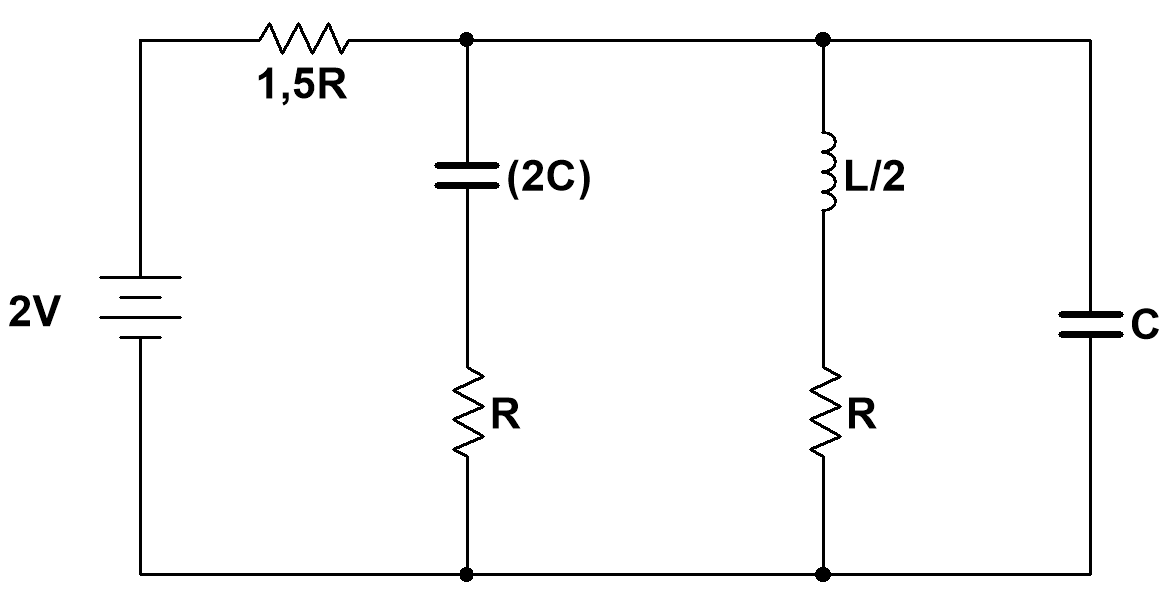
\includegraphics[scale=0.25]{Circuito_2-5.PNG}
	\caption{Circuitos 2.3}
\end{figure}

\begin{flushright}
    $\Box$
\end{flushright}
\newpage
% ----------------------------------------------------------
% QUESTÃO 2.7
% ----------------------------------------------------------
\section*{Questão 2.7}
\addcontentsline{toc}{section}{Questão 2.7}
No Circuito 2.7, seja $i_S = 60e^{-200t} mA$ com $i_1(0)=20mA$.
\begin{itemize}
    \item $(a)$ Calcule $v(t)$ para todo $t$.
    \item $(b)$ Calcule $i_1(t)$ para todo $t\ge0$.
    \item $(c)$ Calcule $i_2(t)$ para todo $t\ge0$. 
\end{itemize}

\begin{figure}[htb]
	\centering
	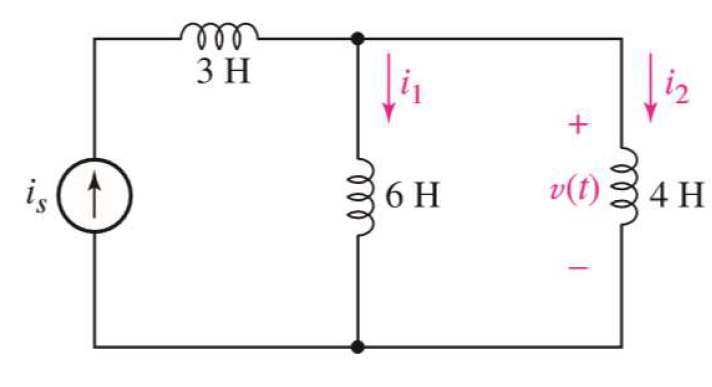
\includegraphics[scale=0.5]{2-7.PNG}
	\caption{Circuitos 2.7}
\end{figure}

Fazendo $t=0$ para $i_S$, obtemos $i_S(0) = 60\,mA$, pois $i_1(0) = 20\,mA$. Logo $i_2(0) = 40\,mA$, sendo essas as condições iniciais do circuito.

Calculando a indutância equivalente entre os indutores $6H$ e $4H$, temos:
$$L_{eq} = 4H \parallel 6H = \dfrac{6H \cdot 4H}{6H + 4H} = 2,4 H$$

%--2.7 - Letra A -------------------------------------------------------------------------------------
$a)$ Assim encontramos $v(t)$ para todo $t$:
$$v(t) = L_{eq} \cdot \dfrac{d i_s(t)}{dt}$$
$$v(t) = 2,4 \cdot (-200)\cdot 60 \times 10^{-3}e^{-200t}$$

\begin{equation}
    \fbox{$v(t) = -28,8e^{-200t}\;V$}
\end{equation}

\newpage

%--2.7 - Letra B -------------------------------------------------------------------------------------
$b)$ Calculando $i_1(t)$ para $t \geq 0$:
$$i_1(t) = \dfrac{1}{L_1}\int_{0}^{t} v(\tau) d\tau + i_1(0)$$
$$i_1(t) = \dfrac{1}{6H}\int_{0}^{t} -28,8e^{-200\tau} d\tau + 20\times10^{-3}$$
$$i_1(t) = 20\times10^{-3}A + \dfrac{-28,8}{6H}\int_{0}^{t} e^{-200\tau} d\tau$$

Fazendo, 
$$
\begin{cases}
u=-200\tau \\
du=-200\;d\tau
\end{cases}
$$

$$i_1(t) = 20\times10^{-3}A + \dfrac{-4,8}{-200}\int_{0}^{t} e^u du$$
$$i_1(t) = 20\times10^{-3}A + 24\times10^{-3}\cdot \left[ e^{-200\tau}\right]_0^t$$
$$i_1(t) = 20\times10^{-3}A + 24\times10^{-3}\cdot (e^{-200t} - e^{-200\cdot 0})$$
$$i_1(t) = 20\times10^{-3}A + 24\times10^{-3}\cdot e^{-200t} - 24\times10^{-3}$$
\begin{equation}
    \centering
    \fbox{$i_1(t) = -4 + 24\cdot e^{-200t}\;mA$}
\end{equation}

%--2.7 - Letra C -------------------------------------------------------------------------------------
$c)$ Calculando $i_2(t)$ para $t \ge 0$:
$$i_2(t) = \dfrac{1}{L_2}\int_{0}^{t} v(t) d\tau + i_2(0)$$
$$i_2(t) = \dfrac{1}{4H}\int_{0}^{t} -28,8e^{-200\tau} d\tau + 40\times10^{-3}$$
$$i_2(t) = 40\times10^{-3}A + \dfrac{-28,8}{4H}\int_{0}^{t} e^{-200\tau} d\tau$$

Fazendo,
$$
\begin{cases}
u=-200\tau \\
du=-200d\tau
\end{cases}
$$

$$i_2(t) = 40\times10^{-3}A + \dfrac{-7,2}{-200}\int_{0}^{t} e^u du$$
$$i_2(t) = 40\times10^{-3}A + 36\times10^{-3}\cdot \left[ e^{-200\tau}\right]_0^t$$
$$i_2(t) = 40\times10^{-3}A + 36\times10^{-3}\cdot (e^{-200t} - e^{-200\cdot 0})$$
$$i_2(t) = 40\times10^{-3}A + 36\times10^{-3}\cdot e^{-200t} - 36\times10^{-3}$$
\begin{equation}
    \centering
    \fbox{$i_2(t) = -4 + 36e^{-200t} mA$}
\end{equation}

\begin{flushright}
    $\Box$
\end{flushright}
\newpage
% ----------------------------------------------------------
% QUESTÃO 2.9
% ----------------------------------------------------------
\section*{Questão 2.9}
\addcontentsline{toc}{section}{Questão 2.9}
Supondo que a chave do Circuito 2.9 tenha estado fechada por um longo tempo, calcule $i_L(t)$ em $(a)$ o instante imediatamente antes de a chave abrir, $(b)$ o instante imediatamente depois de a chave abrir, $(c) t=15.8\mu s$, $(d) t=31.5\mu s$, $(e) t=78.8\mu s$.

\begin{figure}[htb]
	\centering
	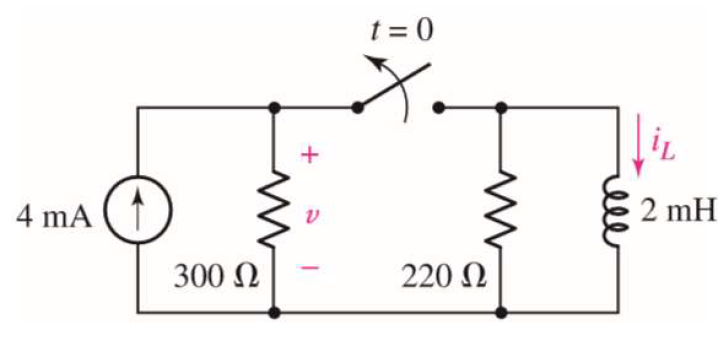
\includegraphics[scale=0.5]{2-9.PNG}
	\caption{Circuitos 2.9}
\end{figure}

%--2.9 - Letra A -------------------------------------------------------------------------------------
$a)$ Encontrando $i_L(t)$ no instante imediatamente antes da chave abrir $I_L(0^-):$

Como o circuito está ligado por bastante tempo, a corrente: $i_L$ é constante e $\dfrac{d i_L}{dt} = 0$, assim:
$$v_L = L\dfrac{d i_L}{dt} \Longrightarrow v_L = L \cdot 0 \Longrightarrow v_L = 0V$$

Como não existe tensão nos terminais do indutor, ele pode ser substituído por um curto-circuito. Desta forma encontramos uma resistência equivalente:
$$\dfrac{1}{R_{eq}}  = \dfrac{1}{300} + \dfrac{1}{220} + \dfrac{1}{0} \Longrightarrow  R_{eq} = 0\Omega$$

Com isso a corrente passa por todo caminho que não possui resistência, assim:
\begin{equation}
    \centering
    \fbox{$i_L = i_f = 4\;mA$}    
\end{equation}

%--2.9 - Letra B -------------------------------------------------------------------------------------
$b)$ Encontrando $i_L(t)$ no instante imediatamente depois de a chave abrir $I_L(0^+):$

Como o indutor se opõe à variação de corrente em seus terminais, desta forma a corrente neste elemento se mantém a mesma, portanto:
\begin{equation}
    \centering
    \fbox{$i_L(0) = I_L(0^-) = I_L(0^+) = 4\;mA$}    
\end{equation}
\newpage

%--2.9 - Letra C -------------------------------------------------------------------------------------
$c)$ Encontrando $i_L(t)$ em $t=15.8\mu s$

Utilizando a \textbf{\textcolor{red}{fórmula da resposta natural}} da corrente do circuito $RL$, temos:
$$i_L(t) = i_L(0) \cdot e^{-\frac{R}{L} \cdot t}$$

Substituindo $R$, $L$ e $i_L(0)$, temos:

$$i_L(t) = 4 \times 10^{-3} \cdot e^{-\dfrac{220\Omega}{2 \times 10^{-3}H} \cdot t}$$
$$i_L(t) = 4 \times 10^{-3} \cdot e^{-110000 \cdot t} A$$

Para $i_L(15.8\mu s)$, temos:

$$i_L(15.8\mu s) = 4 \times 10^{-3} \cdot e^{-110000 \cdot 15,8 \times 10^{-6}}\;A$$
\begin{equation}
    \centering
    \fbox{$i_L(15.8\;\mu s) = 703\;\mu A$}   
\end{equation}

Da mesma forma, obtemos:

$d)$ Em $t=31,5\;\mu s$
\begin{equation}
    \centering
    \fbox{$i_L(31.5\;\mu s) = 125,10\;\mu A$}   
\end{equation}

$d)$ Em $t=78,8\;\mu s$
\begin{equation}
    \centering
    \fbox{$i_L(78.8\;\mu s) = 688,01\;nA$}  
\end{equation}

\begin{flushright}
    $\Box$
\end{flushright}
\newpage

% ----------------------------------------------------------
% QUESTÃO 2.11
% ----------------------------------------------------------
\section*{Questão 2.11}
\addcontentsline{toc}{section}{Questão 2.11}
Com base no circuito 2.11, calcule as correntes $i_{1}$ e $i_{2}$ em $t$ igual a: $(a) 1 ms$, $(b) 3 ms$.

\begin{figure}[htb]
	\centering
	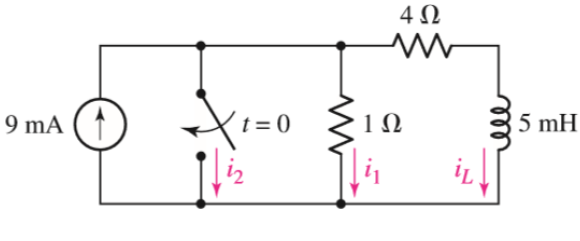
\includegraphics[scale=0.6]{2-11.PNG}
	\caption{Circuito 2.11}
\end{figure}

Calculando $i_L(0^-)$=$i_L(0)$=$i_L(0^+)$:

No regime a corrente no indutor é constante e a tensão entre seus terminais é $0V$, logo ela pode ser considerada como um curto. Então $i_L$ será dada pela corrente em $R_2 = 4 \Omega $. Utilizando \textbf{\textcolor{red}{divisor de corrente}}, temos:

$$i_L(0^-) = \dfrac{R_1}{R_1 + R_2} \cdot I_{tot} $$
$$i_L(0^-) = \dfrac{1}{1 + 4} \cdot 9 mA = 1,8\;mA$$

Com a chave fechada, o circuito resultante é \textbf{\textcolor{red}{resposta natural}} com o resistor de $4 \Omega$ e o indutor de $5 mH$. Logo, pode-se obter a expressão da corrente no indutor pela fórmula:
$$ i_L(t) = i_{f} + (i_{i} - i_{f})\cdot e^{{-\dfrac{R}{L}}\cdot t} $$
$$ i_L(t) = 0 + (-1,8 - 0)\cdot e^{-\dfrac{4}{5\cdot10^{-3}}\cdot t} $$
\begin{center}
    $i_L(t) = -1,8e^{-800\cdot t} mA$     para    $t \ge 0$
\end{center}

%--2.11 - Letra A ---------------------------
$a)$ Em $t = 1\;ms$, por \textbf{\textcolor{red}{LCK}}: $i_2 = i_f + i_L$, temos que:
$$ i_L(1\;ms) = -1,8e^{-800\cdot 1 \cdot 10^{-3}} mA$$
$$i_L(1\;ms) = -808,792 \mu A$$
\begin{equation}
    \fbox{$i_1(1\;ms) = 0 A$}
\end{equation}
\begin{equation}
\fbox{$i_2(1\;ms) = 9 - 0,808 = 8,192\;mA$}
\end{equation}

\newpage %Pula para próxima página forçadamente

%--2.11 - Letra B ----------------------------
$b)$ Em $3 ms$, temos:

$$ i_L(3 ms) = -1,8e^{-800\cdot 3 \cdot 10^{-3}}mA $$
$$i_L(3 ms) = -163 \;\mu A$$
\begin{equation}
    \fbox{$i_1(3 ms) = 0\;A$}
\end{equation}
\begin{equation}
\fbox{$i_2(3\;ms) = 9 - 0,163 = 8,837\;mA$}
\end{equation}

\begin{flushright}
    $\Box$
\end{flushright}
\newpage
% ----------------------------------------------------------
% QUESTÃO 2.13
% ----------------------------------------------------------

\section*{Questão 2.13}
\addcontentsline{toc}{section}{Questão 2.13}
Para o Circuito 2.13, $(a)$ determine $v_L(0^-)$, $v_L(0^+)$, $i_L(0^-)$ e $i_L(0^+)$; $(b)$ Calcule $i_L(150\;ns)$.

\begin{figure}[htb]
	\centering
	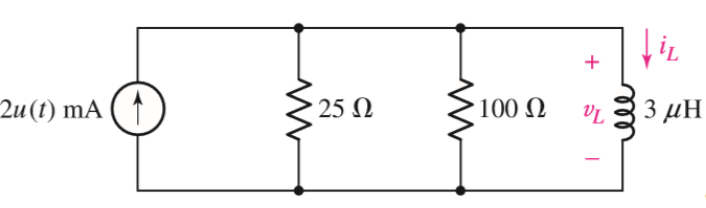
\includegraphics[scale=0.5]{2-13.PNG}
	\caption{Circuito 2.13}
\end{figure}
%--2.13 - Letra A ----------------------------
$(a)$ Determinando $v_L(0^-)$, $v_L(0^+)$, $i_L(0^-)$ e $i_L(0^+)$

Para $t < 0$, a fonte de corrente está \textbf{ABERTA}, portanto a corrente no indutor no instante anterior ao chaveamento do circuito é: $i_L(0^-)=0A$. Como o indutor se opõe à variação de corrente em seus terminais, o valor no instante após o chaveamento é: 
\begin{equation}
    \centering
    \fbox{$i_L(0^-)=i_L(0^+)=0\;A$}
\end{equation}

A tensão no indutor no instante antes do chaveamento é: $v_L{(0^-)} = 0\;V$.

Já no instante após o chaveamento, como o indutor se opõe a variação de corrente em seus terminais, a corrente da fonte de corrente se divide nos resistores, por \textbf{\textcolor{red}{divisor de corrente}}, temos:
\begin{equation}
    \centering
    \fbox{$i_1(0^+) = \dfrac{100}{100 + 25} \cdot 2\;mA = 1,6\;mA$}
\end{equation}
\begin{equation}
    \centering
    \fbox{$v_L(0^+) = R_{25 \Omega} \cdot i_1(0^+) = 40\;mV$}
\end{equation}

\newpage
%--2.13 - Letra B ----------------------------
$b)$ Calculando a constante de tempo do circuito, temos:
$$ \tau = \dfrac{L}{R_{eq}} = \dfrac{3 \;\mu H}{100 \Omega \parallel 25 \Omega} = \dfrac{3 \times 10^{-6}}{20} = 150 ns$$

Como $\tau=150\;ns$, o indutor já possui 63,2\% da sua corrente final, que em breve analise do circuito, sabemos que será igual a corrente da fonte de corrente. Com isso, a corrente em $i_L{(150\;ns)}$ é igual a:

$$i_L{(150\;ns)} = I_f \cdot [1-e^{\left(\dfrac{-t}{\tau}\right)}]A$$
$$i_L{(150\;ns)} = 2 \cdot (1-e^{-1})mA$$
$$i_L{(150\;ns)} = 2 \cdot 0,632 \; mA$$
\begin{equation}
    \centering
    \fbox{$i_L{(150\;ns)} = 1,264 \; mA$}
\end{equation}

\begin{flushright}
    $\Box$
\end{flushright}
\newpage
% ----------------------------------------------------------
% QUESTÃO 2.15
% ----------------------------------------------------------

\section*{Questão 2.15}
\addcontentsline{toc}{section}{Questão 2.15}
Para o Circuito 2.15, observe que uma fonte está sempre ligada. $(a)$ Obtenha uma expressão para $i(t)$ válida para todo $t$.

\begin{figure}[htb]
	\centering
	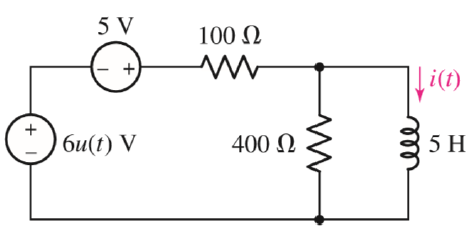
\includegraphics[scale=0.60]{2-15.PNG}
	\caption{Circuito 2.15}
\end{figure}

Para $t<0$ (Regime 1):
Removendo $L$ e calculando o \textbf{\textcolor{red}{equivalente de Thévenin}}, temos:
$$V_{TH} = \dfrac{400\Omega}{100\Omega+400\Omega} \cdot 5\;V = 4\;V$$
$$R_{TH} = 100\Omega \parallel 400 \Omega = \dfrac{100\Omega \cdot 400\Omega}{100\Omega+400\Omega} = 80\;\Omega$$

Assim,
\begin{figure}[htb]
	\centering
	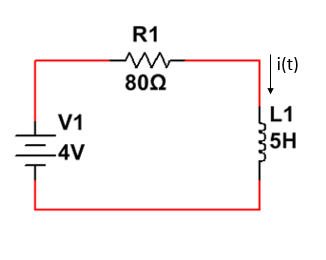
\includegraphics[scale=0.60]{Circuito_2-15(a).PNG}
\end{figure}

No regime 1, a corrente no indutor $I_0$ é:
$$I_0 = \dfrac{V_{TH}}{R_{TH}} = \dfrac{4\;V}{80\;\Omega} = 50\;mA$$
\newpage

Para $t>0$ (Regime 2):
Calculando novamente o \textbf{\textcolor{red}{equivalente de Thévenin}}, temos:
$$R_{TH} = 80\;\Omega$$

Por \textbf{\textcolor{red}{Divisor de tensão}}, obtemos:
$$V_{TH} = \dfrac{400\Omega}{100\Omega+400\Omega} \cdot 11\;V = 8,8\;V$$

No regime 2, a corrente no indutor $I_f$ é:
$$I_f = \dfrac{V_{TH}}{R_{TH}} = \dfrac{8,8\;V}{80\;\Omega} = 110\;mA$$

Calculando a \textbf{\textcolor{red}{resposta à um degrau}} RL:

$$i(t) = I_f+(I_0-I_f) \cdot e^{- \tau^{-1} \cdot t}$$
$$\tau^{-1} = \dfrac{R}{L} = \dfrac{80}{5} = 16\;s^{-1} \Longrightarrow \tau = 62,5\;ms$$
$$i(t) = 110 \cdot 10^{-3}+(50 \cdot 10^{-3}-110 \cdot 10^{-3}) \cdot e^{- t/62,5\cdot 10^{-3}}$$
\begin{equation}
    \centering
    \fbox{$i(t) = 110 - 60e^{-16t}\;mA$}
\end{equation}

\begin{flushright}
    $\Box$
\end{flushright}
\newpage

% ----------------------------------------------------------
% QUESTÃO 2.17
% ----------------------------------------------------------

\section*{Questão 2.17}
\addcontentsline{toc}{section}{Questão 2.17}
Obtenha uma expressão para $i_1$ conforme indicado no Circuito 2.17 que é válida para todos os valores de t.
\begin{figure}[htb]
	\centering
	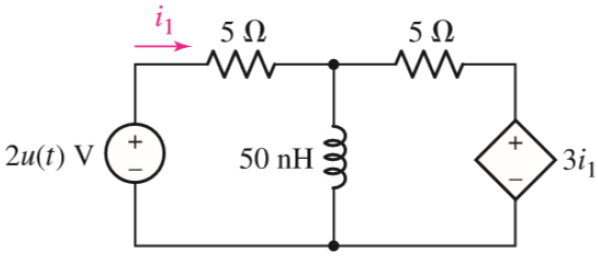
\includegraphics[scale=0.5]{2-17.PNG}
	\caption{Circuito 2.17}
\end{figure}

($Para \; t>0$). Como o indutor está descarregado,
$\begin{cases}
i_1 = 0A \\
i_L = 0A
\end{cases}$

Para $t>>0$ (Regime 2), temos:
\begin{figure}[htb]
	\centering
	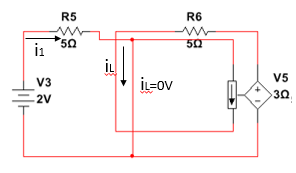
\includegraphics[scale=1]{Circuito_2-17(b).PNG}
\end{figure}

Aplicando \textbf{\textcolor{red}{LTK na Malha 1}}, temos:
$$-2+5i_1=0$$
$$i_1(\infty)=\dfrac{2}{5}=400\;mA$$

Para ${t\geq{0^+}}$, temos:

\begin{figure}[htb]
	\centering
	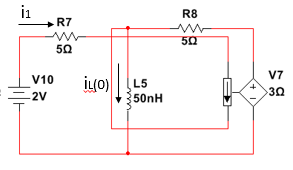
\includegraphics[scale=1]{Circuito_2-17(c).PNG}
\end{figure}

\newpage

Aplicando \textbf{\textcolor{red}{LTK na Malha Externa}}

$$-2+5i_1(0^+)+5i_1(0^+)+3i_1(0^+)=0$$
$$i_1(0^+)=\dfrac{2}{13}=153,846\;mA$$

Calculando $R_{TH}$, sabendo que:
$\begin{cases}
    I_1=i_1\\
    I_2=-i_t
\end{cases}$

\begin{figure}[htb]
	\centering
	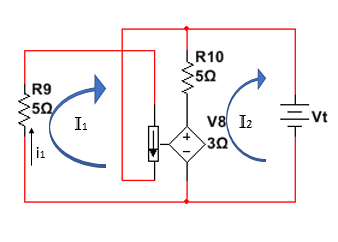
\includegraphics[scale=0.8]{Circuito_2-17(d).PNG}
\end{figure}

Fazendo a \textbf{\textcolor{red}{Análise na Malha 1}}, temos:
$$5I_1+5(I_1-I_2)+3I_1=0$$
$$13I_1-5I_2=0$$

Fazendo a \textbf{\textcolor{red}{Análise na Malha 2}}, temos:
$$-3I_1+5(I_2-I_1)+V_t=0$$
$$-8I_1-5I_2=-V_t$$
Obtemos o seguinte sistema de equações:
$\begin{cases}
    13I_1 - 5I_2= 0 \\
    -8I_1 - 5I_2= -V_t
\end{cases}$, assim: 

$$-13V_t=-25i_t$$
$$R_{TH}=\dfrac{V_t}{i_t}=\dfrac{25}{13}=1,9230\;\Omega$$
$$\tau=\dfrac{L}{R_{TH}}=\dfrac{50\times10^{-9}}{1,9230}=26\;ns$$

\begin{equation}
    \centering
    \fbox{$i_1(t)=400-246,154e^{\dfrac{-t}{\tau}} \;mA$}
\end{equation}

\begin{flushright}
    $\Box$
\end{flushright}
\newpage

% ----------------------------------------------------------
% QUESTÃO 2.19
% ----------------------------------------------------------

\section*{Questão 2.19}
\addcontentsline{toc}{section}{Questão 2.19}
A chave do Circuito 2.19 esteve fechada por um tempo extremamente longo antes de ser aberta em $t=0$. Calcule a corrente indicada por $i_x$ em $t=70\;ms$.

\begin{figure}[htb]
	\centering
	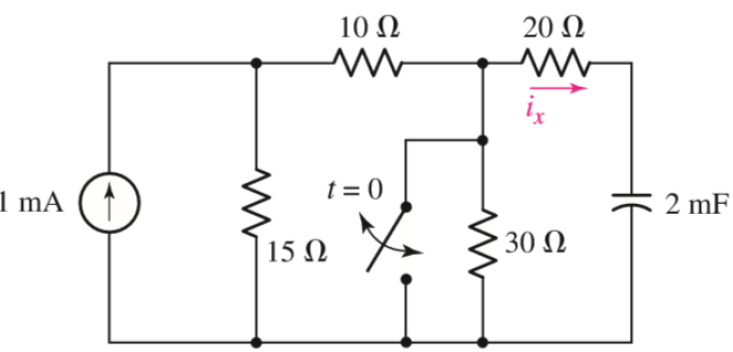
\includegraphics[scale=0.5]{2-19.PNG}
	\caption{Circuito 2.19}
\end{figure}

Com $t<0$, o capacitor e o resistor de 20 $\Omega$ estão em curto-circuito, portanto o capacitor está descarregado. Em $t=0$, calculando as variáveis para encontrar a expressão da corrente, tem-se que:

\begin{figure}[htb]
	\centering
	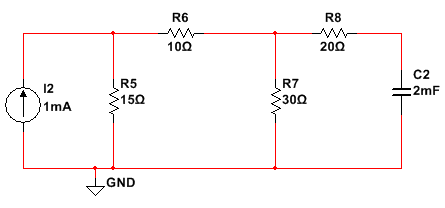
\includegraphics[scale=0.75]{Circuito_2-19(a).PNG}
\end{figure}

Removendo o capacitor para podermos calcular o \textbf{\textcolor{red}{equivalente de Thévenin}}, é possível encontrar $V_{TH}$, fazendo \textbf{\textcolor{red}{transformações de fontes}}, assim:
\begin{figure}[htb]
	\centering
	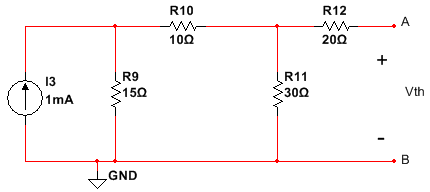
\includegraphics[scale=0.75]{Circuito_2-19(c).PNG}
\end{figure}

\newpage

Transformando para fonte de tensão $V_1 = 15 \Omega \cdot 1 \times 10^{-3}\;A = 15 \; mV$, assim:

\begin{figure}[htb]
	\centering
	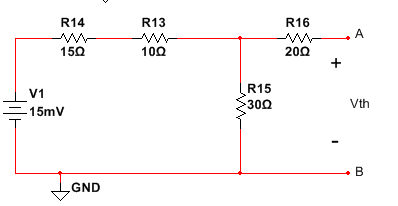
\includegraphics[scale=0.8]{Circuito_2-19(d).PNG}
\end{figure}

Sendo possível calcular o \textbf{\textcolor{red}{equivalente de Thévenin}} por \textbf{\textcolor{red}{divisor de tensão}}:

$$V_{TH} = \dfrac{30}{15+10+30} \cdot 15 \;mV \Longrightarrow V_{TH} = 8,182 \; mV$$ 

A resistência de Thévenin pode ser encontrada \textbf{\textcolor{red}{removendo-se a fonte de tensão}}, desta forma a fonte de tensão perde seu efeito, assim:

\begin{figure}[htb]
	\centering
	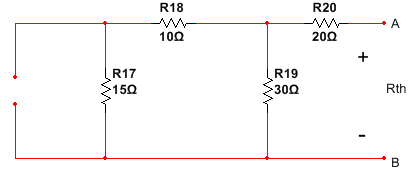
\includegraphics[scale=0.75]{Circuito_2-19(e).PNG}
\end{figure}

$$R_{TH} = \dfrac{(15\Omega+10\Omega) \cdot 30\Omega}{(15\Omega+10\Omega) + 30\Omega} + 20 \Omega \Longrightarrow R_{TH} = 33,636 \; \Omega$$

Transformando o circuito equivalente de Thévenin para o circuito equivalente de Norton e colocando o capacitor de volta ao circuito, temos:
$$I_{NT} = V_{TH} \cdot R_{TH} \Longrightarrow I_{NT} = 1,182\;mV \cdot 33,636\;\Omega \Longrightarrow I_{NT} = 243\;mA$$
$$R_{NT}=R_{TH}=33,636\;\Omega$$

\begin{figure}[htb]
	\centering
	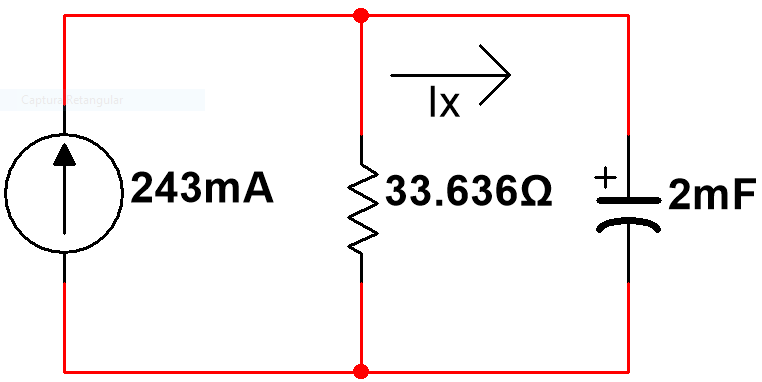
\includegraphics[scale=0.3]{Circuito_2-19(g).PNG}
\end{figure}

Calculando a constante de tempo $\tau$, temos:
$$\tau=R \cdot C \Longrightarrow \tau=33,636\;\Omega \cdot 2\cdot 10^{-3}\;F \Longrightarrow \tau = 67,273\;ms$$


A expressão de $i_x$ é dada por $i_x(t)=I_n \cdot e^{-\dfrac{t}{\tau}}\;para\;t>0$, assim:
$$i_x(70\;ms)=243 \cdot e^{-\dfrac{70\times10^{-3}}{67,273\times10^{-3}}}\;\mu A$$
\begin{equation}
    \fbox{$i_x(70\;ms)=86 \;\mu A$}
\end{equation}

\begin{flushright}
    $\Box$
\end{flushright}
\newpage
% ----------------------------------------------------------
% QUESTÃO 2.22
% ----------------------------------------------------------

\section*{Questão 2.22}
\addcontentsline{toc}{section}{Questão 2.22}
Para um determinado circuito $RLC$ paralelo sem fonte, $R=1\;k\Omega$, $C = 3\;\mu F$, e $L$ é tal que a resposta do circuito é sobre-amortecida. $(a)$ Determine o valor de $L$. $(b)$ Escreva a equação para a tensão $v$ sobre o resistor, sabendo-se que $v(0^-) = 9\;V$ e $\dfrac{dv}{dt} \Bigg|_{t=0^+}^{} = 2 \;V/s$.

%--2.22 - Letra A ----------------------------
$a)$ Como a resposta do circuito é superamortecida, temos que:
$${\dfrac{1}{RC}}>{\dfrac{1}{\sqrt{LC}}}$$
$${\dfrac{1}{1\cdot10^3\cdot3\cdot10^-6}}>{\dfrac{1}{\sqrt{L\cdot3\cdot(10^-6)}}}$$
$$L>12\;H$$

Como a resposta do circuito é \textcolor{red}{superamortecida}, a solução da tensão é dada por:
$$v=A_1e^{s_1\cdot t}+A_2e^{s_2\cdot t}\;V$$

Calculando $s_1$ e $s_2$:
$$s_1=-\alpha+\sqrt{\alpha^2-\omega_0^2}\; rad/s$$
$$s_2=-\alpha-\sqrt{\alpha^2-\omega_0^2}\; rad/s$$

Assumindo $L=13H$, temos:
$$s_1,s_2=\dfrac{-1}{2\times10^3\times3\times10^-6}\pm\sqrt{\left(\dfrac{1}{6\cdot10^-3}\right)^2-\left(\dfrac{1}{13\cdot3\cdot10^-6}\right)^2}$$
$$s_1=-120,442 \;rad/s$$
$$s_2=-212,894 \;rad/s$$

Como o capacitor se opõe a variação de tensão $v(0^-)$=$v(0^+)$=9\;V
$$\dfrac{dv(0^+)}{dt}=2\;V/s$$

$\begin{cases}
A_1+A_2=v(0^+) \\
-120,442\cdot A_1-212,892\cdot A_2=2
\end{cases}$
$$A_1=20,7467\;V e \;A_2=-11,7467\;V$$

%--2.22 - Letra B ----------------------------
Assim, a equação para a tensão $v$ sobre o resistor é:
\begin{equation}
    \centering
    \fbox{$v(t) = 20,747\times e^{-120,442\cdot t} - 11,747\times e^{-212,892\cdot t}\;V$}
\end{equation}

\begin{flushright}
    $\Box$
\end{flushright}
\newpage

% ----------------------------------------------------------
% QUESTÃO 2.24
% ----------------------------------------------------------

\section*{Questão 2.24}
\addcontentsline{toc}{section}{Questão 2.24}
A corrente que circula por um resistor de $5\;\Omega$ em um circuito $RLC$ paralelo sem fonte é determinada por $i_R(t) = 2e^{-t}-3e^{-8t}\;A$, $t > 0$. Determine a corrente máxima e o momento em que ela ocorre.

A corrente máxima ocorre quando:

$$\dfrac{di_R(t)}{dt} = 0$$

Assim, encontramos a derivada de $i_R(t)$ e igualamos a zero:
$$-2\cdot e^{-t}+24\cdot e^{-8t} = 0$$
$$2\cdot e^{-t} = 24\cdot e^{-8t}$$
$$e^{-t} = 12\cdot e^{-8t}$$
$$ln(e^{-t}) = ln(12)+ln(e^{-8t})$$
$$-t = -8t + ln(12)$$
$$7t=2,484907$$
$$t=0,354987\;s$$
\begin{equation}
    \centering
    \fbox{$t=354,987\;ms$}
\end{equation}

Calculando  $i_R(t)$ em $t=354,987\;ms$, temos:
$$i_R(354,987\;ms) = 2e^{-354,987\times10^{-3}}-3e^{-8\cdot354,987\times10^{-3}}\;A$$
$$i_R(354,987\;ms) = 1,402 - 0,175$$
\begin{equation}
    \centering
    \fbox{$i_{max} = i_R(354,987\;ms) = 1,227\;A$}
\end{equation}

\begin{flushright}
    $\Box$
\end{flushright}

\newpage

% ----------------------------------------------------------
% QUESTÃO 2.26
% ----------------------------------------------------------

\section*{Questão 2.26}
\addcontentsline{toc}{section}{Questão 2.26}
Obtenha expressões para a corrente $i(t)$ e a tensão $v(t)$ indicadas no Circuito 2.26 que são válidas para todo $t > 0$. 
\begin{figure}[htb]
	\centering
	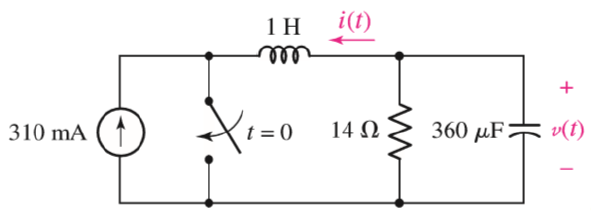
\includegraphics[scale=0.65]{2-26.PNG}
	\caption{Circuito 2.26}
\end{figure}

Calculando $\alpha$ e $\omega_0$:
$$\alpha = \dfrac{1}{2RC} = \dfrac{1}{2\cdot14\cdot360\times10^{-6}} = 99,2063 \;rad/s$$
$$\omega_0 = \dfrac{1}{\sqrt{LC}} = \dfrac{1}{\sqrt{1\cdot360\times10^{-6}}} = 52,7046 \;rad/s$$

Como  $\alpha > \omega_0$, o circuito possui resposta \textbf{\textcolor{red}{superamortecida}}, onde: 
$$v(t)=A_1e^{s_1t} + A_2e^{s_2t}\;V$$

Calculando $s_1$ e $s_2$, em que:
$\begin{cases}
    s_1=-\alpha + \sqrt{\alpha^2-\omega_0^2}\;rad/s\\
    s_2=-\alpha - \sqrt{\alpha^2-\omega_0^2}\;rad/s
\end{cases}$

$$s_1=-99,2063 + \sqrt{(99,2063)^2-(52,7046)^2} \Longrightarrow s_1=-15,158 \;rad/s$$
$$s_2=-99,2063 - \sqrt{(99,2063)^2-(52,7046)^2} \Longrightarrow s_2=-183,255 \;rad/s$$

Para calcular $A_1$ e $A_2$, é necessário encontrar $v(0^+)$ e $\dfrac{dv(0^+)}{dt} = \dfrac{di_C(0^+)}{C}$:
$$v_C(0^-) = v_C(0^+) = 14\cdot310\times10^{-3} = 4,34\;V$$

Com isso, temos que:
\begin{equation}
    \centering
    v(0^+) = A_1 + A_2
    \label{eq1_2.26}
\end{equation}

A corrente no indutor $i_L(0^-)$ é:
$$i_L(0^-) = i_L(0^+) = -310\;mA$$

Como o capacitor mantém sua tensão em paralelo, $i_R(0^+) = \dfrac{4,34\;V}{14\Omega}=310\;mA$
\newpage
Aplicando \textbf{\textcolor{red}{LCK}}, tems que:
$$-i_C(0^+) + i_R(0^+) + i_L(0^+) = 0$$
$$i_C(0^+) = 310\;mA - 310\;mA \Longrightarrow i_C(0^+) = 0 A$$

$$\dfrac{di_C(0^+)}{C} = A_1s_1+A_2s_2 = 0$$
\begin{equation}
    \centering
    -A_1\cdot15,158 - A_2\cdot183,255 = 0
    \label{eq2_2.26}
\end{equation}

As equações~\eqref{eq1_2.26} e~\eqref{eq2_2.26} formam o sistema a ser resolvido:

$\begin{cases}
    A_1 + A_2 = 4,34\;V\\
    -A_1\cdot15,158 - A_2\cdot183,255 = 0
\end{cases}$

Resolvendo, temos:
$$A_1=4,731\;V \; e \; A_2=-0,3914\;V$$

Assim obtemos $v(t)$ para todo $t\geq0$:
\begin{equation}
    \centering
    \fbox{$v(t) = 4,731e^{-15,158t} - 0,3914e^{183,255} \; V$}
\end{equation}

Calculamos $i_R(t)$ e $i_C(t)$ para encontrarmos $i_L(t)$ que é a corrente que passa no indutor (para $t\geq0$):
$$i_R(t) = \dfrac{v(t)}{14\Omega} = 337,954e^{-15,158t} - 27,954e^{-183,255} \; mA$$
$$i_C(t) = C\dfrac{dv}{dt} = 360\times10^{-3}\cdot\left(-71,718e^{-15,158t} + 71,718e^{-183,255}\right) \; mA$$
$$i_C(t) = -25,818e^{-15,158t} + 25,818e^{-183,255} \; mA$$

Sabendo que $i_L(t) = i_R(t) - i_C(t)$, assim:
\begin{equation}
    \centering
    \fbox{$i_L(t) = i(t) = -312,136e^{-15,158t} + 2,136e^{-183,255} \; mA$}
\end{equation}


\begin{flushright}
    $\Box$
\end{flushright}
\newpage

% ----------------------------------------------------------
% QUESTÃO 2.28
% ----------------------------------------------------------

\section*{Questão 2.28}
\addcontentsline{toc}{section}{Questão 2.28}
Para o Circuito 2.28, considere $i_s(t) = 10u(-t)\;A$. $(a)$ Selecione $R_1$ para que $v(0^+)=6\;V$. $(b)$ Calcule $v(2\;ms)$. $(c)$ Determine o tempo de acomodação da tensão no capacitor. $(d)$ O tempo de acomodação da corrente no indutor é o mesmo da sua resposta para o item $(c)$?
\begin{figure}[htb]
	\centering
	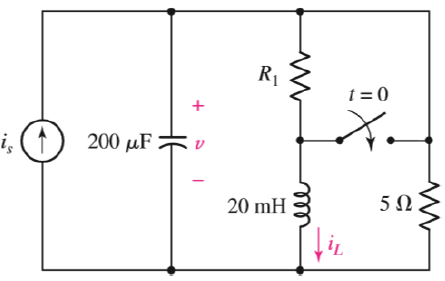
\includegraphics[scale=0.7]{2-28.PNG}
	\caption{Circuito 2.28}
\end{figure}

%--2.28 - Letra a ----------------------------
$a)$ Sabemos que $v(0^+) = 6\;V = v(0^-)$, assim:
$$i_R(0^-) = i_s(0^-) - i_{5\Omega}(0^-)$$
$$i_R(0^-) = 10 - \dfrac{6\;V}{5\;\Omega} = 8,8\;A$$
\begin{equation}
    \centering
    R_1 = \dfrac{v(0^-)}{i_{R_1}(0^-)} = \dfrac{6\;V}{8,8\;A} \Longrightarrow \fbox{$R_1 = 681,\overline{81}\;m\Omega$}
\end{equation}

%--2.28 - Letra b ----------------------------
$b)$ Retirando a fonte de corrente e observando que quando a chave está fechada um curto-circuito elimina o resistor $R_1$, assim:

\begin{figure}[htb]
	\centering
	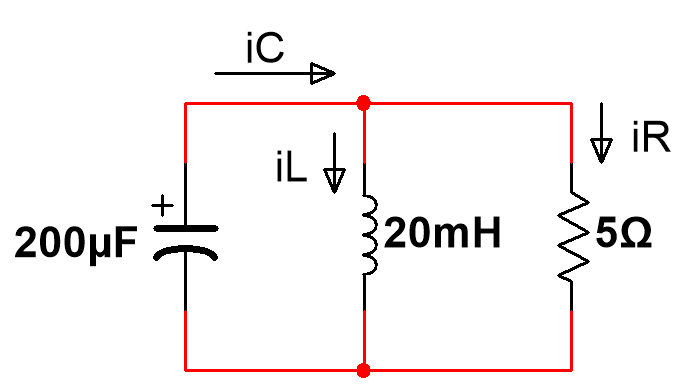
\includegraphics[scale=0.35]{Circuitos_2-28.PNG}
\end{figure}

Calculando $\alpha$ e $\omega_0$, temos:
$$\alpha = \dfrac{1}{2RC} = \dfrac{1}{2\cdot5\cdot200\times10^{-6}} = 500 \;rad/s$$
$$\omega_0 = \dfrac{1}{\sqrt{LC}} = \dfrac{1}{\sqrt{20\times10^{-3}\cdot360\times10^{-6}}} = 500 \;rad/s$$
\newpage
Como $\alpha=\omega_0$, a resposta do circuito é \textbf{\textcolor{red}{criticamente amortecida}} e a equação da tensão, neste caso, é dada por:
$$v(t) = (D_1t+D_2)e^{-\alpha t} \; V \;\; para \;\; t\geq0$$
$$v(0^+) = v_0 = D_2 = 6\;V$$
$$\dfrac{d(0^+)}{dt} = \dfrac{i_C(0^+)}{C} = D_1 - \alpha D_2$$
$$\dfrac{-[i_L(0^+)+i_R(0^+)]}{200\times10^{-6}} = D_1 - 500\cdot6 \Longrightarrow D_1 = 47000$$
$$v(t) = (-47000t + 6)e^{-500t}\;V$$

Calculando $v(t)$ para $t=2\;ms$, temos:
$$v(2\;ms) = (-47000\cdot2\times10^{-3} + 6)e^{-500\cdot2\times10^{-3}} \;V$$
\begin{equation}
    \centering
    v(2\;ms) = -32,373\;V
\end{equation}

%--2.28 - Letra c ----------------------------
$c)$ Calculando o tempo de acomodação da tensão no capacitor:
$$t_S = \dfrac{4}{\tau \cdot \omega_0}\;\;(\textcolor{red}{crit\acute{e}rio\;dos\;2\%})$$
$$\tau = \dfrac{RC}{2} \cdot \sqrt{\dfrac{1}{LC}}$$
$$t_S = \dfrac{4}{\dfrac{5\cdot 200\times10^{-6}}{2} \cdot \sqrt{\dfrac{1}{20\times10^{-3}\cdot200\times10^{-6}}} \cdot 500}$$
\begin{equation}
    \centering
    \fbox{$t_S = 32 ms$}
\end{equation}

%--2.28 - Letra d ----------------------------
$d)$ O tempo de acomodação da corrente no indutor é o mesmo da sua resposta para o item $(c)$ pois o mesmo depende somente de $R,L\;e\;C$

\begin{flushright}
    $\Box$
\end{flushright}
\newpage

% ----------------------------------------------------------
% QUESTÃO 2.30
% ----------------------------------------------------------

\section*{Questão 2.30}
\addcontentsline{toc}{section}{Questão 2.30}
Para o Circuito 2.30, determine $(a)$ a primeira vez $t > 0$ quando $v(t) = 0$; $(b)$ o tempo de acomodação. 
\begin{figure}[htb]
	\centering
	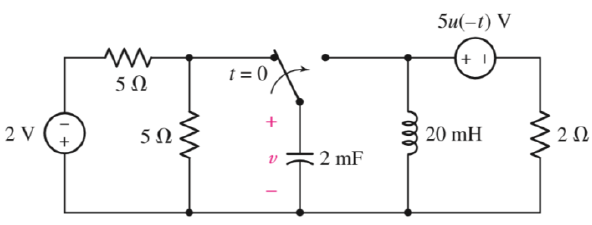
\includegraphics[scale=0.7]{2-30.PNG}
	\caption{Circuito 2.30}
\end{figure}

Para $t<0$, temos:

Aplicando divisor de tensão, no lado esquerdo do circuito
$$v_C(0^-)=\dfrac{R_1}{R_1+R_2}\cdot V_{total} $$
$$v_C(0^-)=\dfrac{5\Omega}{5\Omega+5\Omega}\cdot-2\;V $$
$$v_C(0^-)=-1\;V$$

Aplicando lei de ohm, no lado direito do circuito
$$i_L(0^-)=\dfrac{V}{R}$$
$$i_L(0^-)=\dfrac{5}{2} = 2,5\;A$$

Em $t\geq0$, com a chave fechando outros dois contatos, obtêm-se um circuito $RLC$, com resposta natural. Natural porque a fonte de tensão do lado direito é $0\;V$. Como não há elemento forçante, o circuito agora é um $RLC$ paralelo.

Calculando $\alpha$(frequência de neper) e $\omega_o$(frequência angular de ressonância), temos:
$$\alpha=\dfrac{1}{2 R C} \Longrightarrow \alpha=\dfrac{1}{2\cdot 2\Omega \cdot 2\cdot10^{-3}F} \Longrightarrow \alpha=125\;rad/s$$
$$\omega_o=\dfrac{1}{\sqrt{L C}} \Longrightarrow \omega_o=\dfrac{1}{\sqrt{20\cdot10^{-3} \cdot 2\cdot10^{-3}}} \Longrightarrow \omega_o=158,114\;rad/s$$
\newpage
Como $\omega_o>\alpha$, logo a resposta é $\textcolor{red}{subamortecida}$. Com isso, a tensão será dada pela seguinte fórmula:
$$v(t)=B_1 e^{-\alpha t} \cos{\omega_d t}\;+\;B_2 e^{-\alpha t} \sen{\omega_d t}\;V$$
$$\omega_d=\sqrt{\omega_o^2-\alpha^2}\;rad/s$$
$$\omega_d=\sqrt{158,114^2-125^2}$$
$$\omega_d=96,8248\;rad/s$$

$$B_1=v(0^-)=v(0)=v(0^+)=-1\;V$$
$$i_R(0^+)=\dfrac{v(0^+)}{R}$$
$$i_R(0^+)=\dfrac{-1\;V}{2\Omega}=-0,5\;A $$

Aplicando \textbf{\textcolor{red}{LCK}}, temos:
$$i_C(0^+)=-i_R(0^+)-i_L(0^+)$$
$$i_C(0^+)=-(-0,5)-2,5\;A$$
$$i_C(0^+)=-2\;A $$

Calculando $B_2$:
$$\dfrac{i_C(0^+)}{C}=-\alpha B_1+\omega_dB_2$$
$$\dfrac{-2}{2\cdot10^{-3}}=-125\cdot(-1)-96,8248B_2$$
$$B_2=-11,6189\;V$$

Logo:
$$v(t)=-e^{-125t}\cos{96,8248t}-11,6189e^{-125t}\sen{96,8248t}\;V$$

\newpage
%--2.30 - Letra A ----------------------------
$a)$ Calculando t pelo \textbf{\textcolor{red}{método numérico da secante}}, com um erro que garante a certeza das duas primeiras casas decimais ($\varepsilon = 10^{-2}$), temos:

\begin{table}[!htb]
	\centering
	\begin{tabular}{c|c|c|c|c|c|c}
		\hline		
		$n$ & $t_0$ & $t_1$ & $g(t_0)$ & $g(t_1)$ & $t_2$ & $g(t_2)$\\
		\hline
		1 & 0 & $0,035$ & -1 & $4,80\times 10^{-2}$ & $3,34\times 10^{-2}$ & $3,17\times 10^{-2} \rightarrow cont$ \\
		\hline
		\hline
		$n$ & $t_1$ & $t_2$ & $g(t_1)$ & $g(t_2)$ & $t_3$ & $g(t_3)$ \\
		\hline
		2 & $0,035$ & $0,033397$ & $0,048004$ & $3,17\times 10^{-2}$ & $3,03\times 10^{-2}$ & $-3,03\times 10^{-2}\rightarrow cont$ \\
		\hline
		\hline
		$n$ & $t_2$ & $t_3$ & $g(t_2)$ & $g(t_3)$ & $t_4$ & $g(t_4)$\\
		\hline
		3 & $0,033397$ & $0,030267$ & $0,031743$ & $-3,31\times 10^{-2}$ & $0,031865$ & $6,42\times 10^{-3}\rightarrow para$ \\
		\hline
	\end{tabular}
	\caption{Tabela de iterações do Método da Secante para a Questão 2.30}
	\label{tabela-1}
\end{table}

Como $g(t_4) < \varepsilon$, para $t>0$, o primeiro $t$ em que $v(t)=0$ é $t_4$, logo:

\begin{equation}
    \fbox{$t=31,865\;ms$}
\end{equation}

%--2.30 - Letra B ----------------------------
$b)$ O tempo de acomodação será dado por:

$$t_s=\dfrac{4}{\tau \cdot \omega_0}$$
$$\tau=\dfrac{RC}{2}\sqrt{\dfrac{1}{LC}}$$
$$t_s=\dfrac{4}{0,3162\cdot158,114}$$

\begin{equation}
    \fbox{$t=80\;ms$}
\end{equation}


\begin{flushright}
    $\Box$
\end{flushright}
\newpage

% ----------------------------------------------------------
% QUESTÃO 2.32
% ----------------------------------------------------------

\section*{Questão 2.32}
\addcontentsline{toc}{section}{Questão 2.32}
Os componentes do Circuito 2.32 possuem os seguintes valores: $R=2\;\Omega$, $C=1\;mF$, e $L=2\;mH$. Se $v_c(0^-)=1\;V$ e inicialmente não circula corrente através do indutor, calcule $i(t)$ nos instantes $t=1\;ms$, $2\;ms$, e $3\;ms$. 
\begin{figure}[htb]
	\centering
	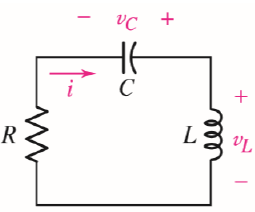
\includegraphics[scale=0.7]{2-32.PNG}
	\caption{Circuito 2.32}
\end{figure}

Calculando $\alpha$ e $\omega_0$ temos:

$$\alpha={\dfrac{R}{2L}}={\dfrac{2}{2\cdot2\times10^-3}}=500 \;rad/s$$
$$\omega_0={\dfrac{1}{\sqrt{LC}}}={\dfrac{1}{\sqrt{2\times10^-3\cdot1\times10^-3}}}=707,107\;rad/s$$

Como $\alpha$ < $\omega_0$, a resposta é subamortecida e tem equação:
$$i(t)=B_1\cdot e^{-\alpha t} \cdot \cos\left(\omega_d\cdot t\right)+ B_2\cdot e^{-\alpha t} \cdot\sen\left(\omega_d\cdot t\right)\;A$$
$$i(0)=B_1=0\;A$$
$${\omega_d=\sqrt{\omega_0^2-\alpha^2}}={\sqrt{707,107^2-500^2}}=500 \;rad/s$$
$${\dfrac{di(0)}{dt}}={\dfrac{v(0)}{L}}=-\alpha B_1+\omega_d B_2={\dfrac{1}{2\times10^{-3}}}=-\alpha\cdot0+500B_2$$
$$B_2=1\;A$$
$$i(t)=e^{-500t}\sen{500t}\;A$$
\begin{equation}
    \fbox{$i(1\;ms)=e^{-500\times10^{-3}}\sen{500\times10^{-3}}=290,786\;mA$}
\end{equation}

\begin{equation}
    \fbox{$i(2\;ms)=e^{-500\cdot2\times10^{-3}}\sen{500\cdot2\times10^{-3}}=309,56\;mA$}
\end{equation}
    
\begin{equation}
    \fbox{$i(3\;ms)=e^{-500\cdot3\times10^{-3}}\sen{500\cdot3\times10^{-3}}=222,571\;mA$}
\end{equation}


\begin{flushright}
    $\Box$
\end{flushright}
\newpage

% ----------------------------------------------------------
% QUESTÃO 2.34
% ----------------------------------------------------------

\section*{Questão 2.34}
\addcontentsline{toc}{section}{Questão 2.34}
Com relação ao Circuito 2.34, calcule $(a) \alpha$; $(b)\omega_0$; $(c)i(0^+)$; $(d)\dfrac{di}{dt}\Bigg|_{0^+}^{}$; $(e)i(t)$ em $t=6\;s$
\begin{figure}[htb]
	\centering
	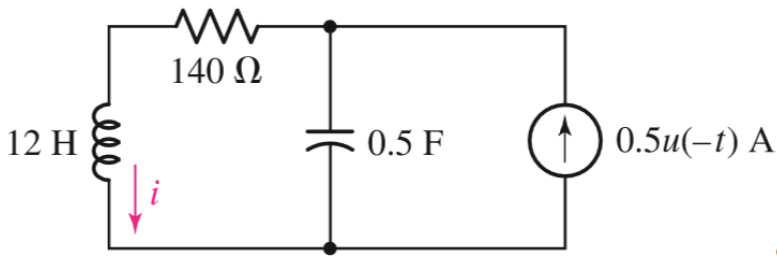
\includegraphics[scale=0.5]{2-34.PNG}
	\caption{Circuito 2.34}
\end{figure}

%--2.34 - Letra A ----------------------------
$a)$ Calculando $\alpha$
$$\alpha={\dfrac{R}{2L}}={\dfrac{140}{2\times12}}= \;5,833rad/s$$

%--2.34 - Letra B ----------------------------
$b)$Calculando $\omega_0$
$$\omega_0={\dfrac{1}{\sqrt{LC}}}={\dfrac{1}{\sqrt{12\cdot0,5}}}=0,4082\;rad/s$$

Como $\alpha$ > $\omega_0$, a resposta do circuito RLC é superamortecida e tem equação:
$$i(t)=A_1e^{s_1\cdot t}+A_2e^{s_2\cdot t}\;A$$

Calculando $s_1$ e $s_2$:
$$s_1=-\alpha+\sqrt{\alpha^2-\omega_0^2}=-5,833+\sqrt{5,833^2-0,4082^2}=-0,01430\;rad/s$$
$$s_2=-\alpha-\sqrt{\alpha^2-\omega_0^2}=-5,833-\sqrt{5,833^2-0,4082^2}=-11,6517\;rad/s$$

%--2.34 - Letra C ----------------------------
$c)$ Calculando $i(0^+)$, temos:
$$i(0^+)=i(0^-)=i(0)=500\;mA$$
$$v(0^-)=70\;V$$

%--2.34 - Letra d ----------------------------
$d)$ Calculando $(d)\dfrac{di}{dt}\Bigg|_{0^+}^{}$, temos::
$${\dfrac{di(0^+)}{dt}}={\dfrac{v(0^+)}{L}}={\dfrac{0}{12}}=0\;A/s$$
\newpage
\begin{equation}
    \centering
    i(0)=A_1+A_2 = 0.5
    \label{eq1_2.34}
\end{equation}

\begin{equation}
    \centering
    {\dfrac{di(0)}{dt}}=s_1A_1+s_2A_2 = -0,01430A_1-11,6517\cdot A_2=0
    \label{eq2_2.34}
\end{equation}

As equações~\eqref{eq1_2.34} e~\eqref{eq2_2.34} formam o sistema a ser resolvido:

$\begin{cases}
A_1+A_2=0.5 \\
-0,01430A_1-11,6517\cdot A_2=0
\end{cases}$

$$A_1=0,500614\;A$$
$$A_2=-0,000614\;A$$

$$i(t)=0,500614e^{-0,01430\cdot t}-0,000614e^{-11,6517\cdot t}\;A$$

%--2.34 - Letra e ----------------------------
$e)$ Calculando $i(t)$ em $t=6\;s$, temos:
$$i(6s)=0,500614e^{-0,01430\times 6}-0,000614e^{-11,6517\times 6}\;A$$

\begin{equation}
    \fbox{$i(6s)=459,450\;mA$}
\end{equation}

\begin{flushright}
    $\Box$
\end{flushright}
\newpage

% ----------------------------------------------------------
% QUESTÃO 2.36
% ----------------------------------------------------------

\section*{Questão 2.36}
\addcontentsline{toc}{section}{Questão 2.36}
Considere o Circuito 2.36. Se $v_s(t) = -8 + 2u(t) V$, determine $(a)v_C(0^+)$, $(b)i_L(0^+)$, $(c)v_C(\infty)$. 

\begin{figure}[htb]
	\centering
	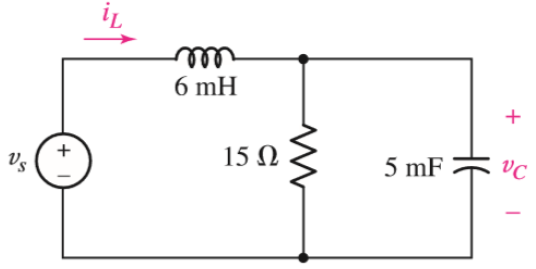
\includegraphics[scale=0.5]{2-36.PNG}
	\caption{Circuito 2.36}
\end{figure}

%--2.36 - Letra a ----------------------------
$a)$Em $t<0$, $V_s$ é igual a $-8\;V$. Dessa forma:
$$V_C(0^-)=V_C(0^+)$$
\begin{equation}
    \fbox{$V_C(0^+)=-8\;V$}
\end{equation}

%--2.36 - Letra b ----------------------------

$b)$A corrente no indutor em $0^+$ é a mesma quando $t<0$, porque o indutor se opõe à variação de corrente em seus terminais, desta forma:
$$i_L(0^-)=i_L(0^+)=\dfrac{V_s}{R}$$
$$i_L(0^+)=\dfrac{-8}{15}$$
\begin{equation}
    \fbox{$i_L(0^+)=-533,333\;mA$}
\end{equation}

%--2.36 - Letra c ----------------------------
$c)$Para $t \rightarrow \infty$, a tensão no capacitor já não irá se opor à variações de tensão. Logo:

\begin{equation}
    \fbox{$V_s(\infty) = V_L(\infty)=-6\;V$}
\end{equation}

\begin{flushright}
    $\Box$
\end{flushright}
\newpage

% ----------------------------------------------------------
% QUESTÃO 2.38
% ----------------------------------------------------------

\section*{Questão 2.38}
\addcontentsline{toc}{section}{Questão 2.38}
Em relação ao Circuito 2.38, $(a)$ obtenha uma expressão para $v(t)$, que é válida para todo $t > 0$; $(b)$ calcule a corrente máxima no indutor e identifique o momento em que ela ocorre; $(c)$ determine o tempo de acomodação. 
\begin{figure}[htb]
	\centering
	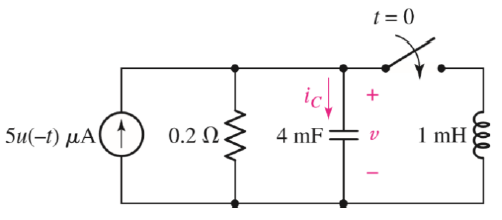
\includegraphics[scale=0.7]{2-38.PNG}
	\caption{Circuito 2.38}
\end{figure}

%--2.38 - Letra a ----------------------------
$a)$ Temos que:
$$v(0^-)=v(0)=0,2\cdot5\cdot10^{-6}=1\;\mu V$$

Para $t>0$ agora há um circuito RLC paralelo, com resposta natural. Calculando as frequências de neper e angular de ressonância:

$$\alpha=\dfrac{1}{2RC} \Longrightarrow \alpha=\dfrac{1}{2\cdot0,2\cdot4\cdot10^{-3}} \Longrightarrow \alpha=625\;rad/s$$

$$\omega_o=\dfrac{1}{\sqrt{LC}} \Longrightarrow \omega_o=\dfrac{1}{\sqrt{1\cdot10^{-3}\cdot 4\cdot10^{-3}}} \Longrightarrow \omega_0=500\;rad/s$$

Como $\alpha$\;>\;$\omega_0$, logo a resposta é $\textcolor{red}{superamortecida}$. Com isso, a tensão será dada pela seguinte fórmula:

$$v(t)=A_1e^{s_1 t}\;+\;A_2e^{s_2 t}\;V$$
$$s_{1}=-\alpha\;+\;\sqrt{\alpha^2-\omega_0^2} \Longrightarrow s_{1}=-625\;+\:\sqrt{625^2-500^2} \Longrightarrow s_{1}=-250\;rad/s$$

$$s_{2}=-\alpha\;-\;\sqrt{\alpha^2-\omega_0^2} \Longrightarrow s_{2}=-625\;-\;\sqrt{625^2-500^2} \Longrightarrow s_{2}=-1000\;rad/s$$

Montando o sistema de equações:
\begin{equation}
    \centering
    v(0)=A_1+A_2 = 0
    \label{eq1_2.38}
\end{equation}
$$i_C(0)=\dfrac{v(0)}{R}=\dfrac{-1\cdot10^{-6}}{0,2}=-5 \mu A$$
$$\dfrac{dv(0)}{dt}=\dfrac{i_C(0)}{C}=s_1A_1\;+\;s_2A_2$$
\begin{equation}
    \centering
    -250A_1-1000A_2 = \dfrac{-5\cdot10^{-6}}{4\cdot10^{-3}}
    \label{eq2_2.38}
\end{equation}

Com as equações~\eqref{eq1_2.38} e~\eqref{eq2_2.38}, podemos encontrando $A_1$ e $A_2$ por meio de sistema de equações, assim é possível encontrar a expressão para a tensão:

$\begin{cases}
    A_1+A_2 = 0 \\
    -250A_1-1000A_2 = \dfrac{-5\cdot10^{-6}}{4\cdot10^{-3}}
\end{cases}$

Sabendo que $A_1=-333.33\;nV\;e\;A_2=1333.33\;nV$, temos:
\begin{equation}
    \fbox{$v(t)=-333,33e^{-250t}\;+\;1333,33e^{-1000t}\;nV$}
\end{equation}

%--2.38 - Letra b ----------------------------
$b)$ Calculando a corrente no indutor, temos:
$$i_L(t)=\dfrac{1}{L}\int_{0}^{t}vd\tau\;i_L(0)$$
$$i_L(t)=\dfrac{1}{10^{-3}}\int_{0}^{t}-333,33e^{-250\tau}\;+\;1333,33e^{-1000\tau}\;nV\;d\tau$$
$$i_L(t)=\dfrac{10^{-9}}{10^{-3}}\int_{0}^{t}-333,33e^{-250\tau}\;+\;1333,33e^{-1000\tau}d\tau$$
$$i_L(t)=10^{-6}(1,333(e^{-250t}-e^0)-1,333(e^{-1000t}-e^0))\;A$$
$$i_L(t)=1,333e^{-250t}-1,333e^{-1000t}\;\mu A$$

Para calcular a corrente máxima, basta calcular a derivada da função $i_L$ e sua raiz:
$$\dfrac{di_L(t)}{dt}=-250\cdot1,333e^{-250t}+1000\cdot\;1,333e^{-1000t}$$

Para $di_L(t)=0$. Logo:
$$333,25e^{-250t}-1333e^{-1000t}=0 \Longrightarrow e^{750t}=4 \Longrightarrow t=\dfrac{\ln{4}}{750}$$
\begin{equation}
    \fbox{$t=1,848\;ms$}
\end{equation}
\begin{equation}
    \fbox{$i_L(1,848ms)=629,803\;nA$}
\end{equation}

%--2.38 - Letra c ----------------------------
$c)$ O tempo de acomodação será dado por:
$$t_s=\dfrac{4}{T\omega_o} \Longrightarrow t_s=\dfrac{4}{500\cdot0,2}\;s$$
\begin{equation}
    \fbox{$t=40\;ms$}
\end{equation}

\begin{flushright}
    $\Box$
\end{flushright}
\newpage

% ----------------------------------------------------------
% QUESTÃO 2.40
% ----------------------------------------------------------

\section*{Questão 2.40}
\addcontentsline{toc}{section}{Questão 2.40}
O Circuito 2.40 sem fonte é construído utilizando um indutor de $10\;mH$, um capacitor de $1\;mF$ e um resistor de $1,5\;k\Omega$. $(a)$ Calcule $\alpha$, $\omega_D$ e $\omega_0$. $(b)$ Determine o valor máximo de $i$ e o tempo em que ele ocorre se o indutor inicialmente não armazena energia e $v(0^-)=9\;V$. 
\begin{figure}[htb]
	\centering
	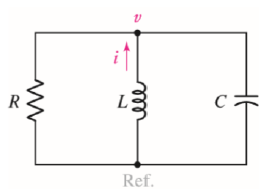
\includegraphics[scale=0.8]{2-40.PNG}
	\caption{Circuito 2.40}
\end{figure}

%--2.40 - Letra a ----------------------------
$a)$ Calculando as frequências de \textit{neper} e angular de ressonância:
\begin{equation}
    \centering
    \alpha=\dfrac{1}{2 R C} \Longrightarrow \alpha=\dfrac{1}{2\cdot1,5\cdot10^3\cdot10^{-3}} \Longrightarrow  \fbox{$\alpha=0,333\;rad/s$}
\end{equation}

\begin{equation}
    \centering
    \omega_o=\dfrac{1}{\sqrt{L C}} \Longrightarrow \omega_o=\dfrac{1}{\sqrt{10\cdot10^{-3}\cdot10^{-3}}} \Longrightarrow \fbox{$\omega_0=316,23\;rad/s$}
\end{equation}

Como $\omega_0>\alpha$, logo a resposta é $\textcolor{red}{subamortecida}$, assim:
\begin{equation}
    \centering
    \omega_d=\sqrt{\omega_o^2-\alpha^2} \Longrightarrow \omega_d=\sqrt{316,23^2-0,333^2} \Longrightarrow \fbox{$\omega_d=316,21\;rad/s$}
\end{equation}

%--2.40 - Letra b ----------------------------
$b)$ Com isso, a tensão será dada pela seguinte fórmula:
$$v(t)=B_1 e^{-\alpha t} \cos{\omega_d t}\;+\;B_2 e^{-\alpha t} \sen{\omega_d t}$$
$$v(0^-)=B_1=9\;V$$

Aplicando \textbf{\textcolor{red}{LCK}}, temos:
$$i_C(0)=-i_R(0)-i_L(0)$$
$$i_C(0)=-\dfrac{9}{1500}-0=-6\cdot10^{-3}\;A$$
$$\dfrac{-6\cdot10^{-3}}{10^{-3}}=-0,333 B_1+316,23B_2$$
$$B_2=-0,00949\;V$$
\newpage
$$v(t)=9 e^{-0,333 t} \cos{316,21 t}\;+\;-0,00949 e^{-0,333 t} \sen{316,21 t} \;V$$

Calculando a expressão da corrente no indutor, temos:
$$i_L(t)=\dfrac{1}{L}\int_{0}^{t}vd\tau\;i_L(0)$$
$$i_L(t)=\dfrac{1}{10\cdot10^{-3}}\int_{0}^{t}9 e^{-0,333\tau} \cos{316,21\tau}-0,00949 e^{-0,333\tau} \sen{316,21 t}d\tau$$

Manipulando matematicamente, temos:
$$i_L(t)=2,846e^{-0,333t}\sen{316,21t}\;+\;3,833\cdot10^{-6}e^{-0,333t}\cos{316,21t}-3,833\cdot10^{-6}\;A$$

Derivando a expressão:
$$\dfrac{di_L(t)}{dt}=-e^{-0,333t}(0,948\sen{316,21t}\;-\;899,93\cos{316,21t})$$

Para $\dfrac{di_L(t)}{dt}=0$ a corrente será máxima. Logo:
$$-e^{-0,333t}(0,948\sen{316,21t}\;-\;899,93\cos{316,21t})=0$$

Calculando t pelo \textbf{\textcolor{red}{método numérico da secante}}, com um erro de 3 casas decimais ($\varepsilon = 10^{-3}$), temos:

\begin{table}[!htb]
	\centering
	\begin{tabular}{c|c|c|c|c|c|c}
		\hline		
		$n$ & $t_0$ & $t_1$ & $g(t_0)$ & $g(t_1)$ & $t_2$ & $g(t_2)$\\
		\hline
		1 & 0 & $6\times 10^{-3}$ & $899,9337$ & $-288,92563$ & $0,004542$ & $119,6646 \rightarrow cont.$ \\
		\hline
		\hline
		$n$ & $t_1$ & $t_2$ & $g(t_1)$ & $g(t_2)$ & $t_3$ & $g(t_3)$ \\
		\hline
		2 & $0,006$ & $0,004542$ & $-288,926$ & $119,664582$ & $0,004969$ & $-1,32148\rightarrow cont.$ \\
		\hline
		\hline
		$n$ & $t_2$ & $t_3$ & $g(t_2)$ & $g(t_3)$ & $t_4$ & $g(t_4)$\\
		\hline
		3 & $0,004542$ & $0,004969$ & $119,6646$ & $-1,32148$ & $0,004964$ & $0,003708\rightarrow cont.$ \\
		\hline
		\hline
		$n$ & $t_3$ & $t_4$ & $g(t_3)$ & $g(t_4)$ & $t_5$ & $g(t_5)$\\
		\hline
		4 & $0,004969$ & $0,004964$ & $-1,32148$ & $0,003708$ & $0,004964$ & $-7,1\times 10^{-9}\rightarrow para$ \\
		\hline
	\end{tabular}
	\caption{Tabela de iterações do Método da Secante para a Questão 2.40}
	\label{tabela-2}
\end{table}

Portanto, o momento em que ocorre a corrente máxima é:
\begin{equation}
    \fbox{$t=4,964\;ms$}
\end{equation}

E a corrente máxima é:
\begin{equation}
    \fbox{$i_{max}=2,841\;A$}
\end{equation}

\begin{flushright}
    $\Box$
\end{flushright}
\newpage
%=====================================================================================================================================================
%=====================================================================================================================================================

% ----------------------------------------------------------
% Finaliza a parte no bookmark do PDF
% para que se inicie o bookmark na raiz
% e adiciona espaço de parte no Sumário
% ----------------------------------------------------------
\phantompart

% ----------------------------------------------------------
% ELEMENTOS PÓS-TEXTUAIS
% ----------------------------------------------------------
\postextual
% ----------------------------------------------------------

% ----------------------------------------------------------
% Referências bibliográficas
% ----------------------------------------------------------
\bibliography{abntex2-modelo-references}

\end{document}
